\documentclass[11pt]{article}
\usepackage[letterpaper, margin=1in]{geometry}
\usepackage[american]{circuitikz}
\usepackage{amsmath}
\usepackage{graphicx}
\usepackage{booktabs}
\usepackage{array}
\usepackage{xcolor}

% 设置段落缩进与间距
\setlength{\parindent}{0pt}
\setlength{\parskip}{0.8em}

\begin{document}

The final project for this course involves the design of the signal conditioning electronics for a strain gage sensor. Your design will amplify amplifier and filter a strain gage signal from a Wheatstone bridge. The project goals are:

\begin{itemize}
    \setlength{\itemsep}{0pt}
    \item Translating application specifications (e.g. dynamic range of a sensor output) into circuit specifications
    \item Assessing different noise sources and their impact in acheiving performance targets (e.g. SNR)
    \item Choosing components for gain and filtering to optimize for SNR, power dissipation, and cost
    \item Evaluating the impact of manufacturing variations on performance goals, and and selecting components that achieve the optimal balance between performance, component availability, and cost
\end{itemize}

The project will consist of two phases. At the end of Phase 1 you are asked to submit a Jupyter Notebook providing details of your design choices and the results of any relevant analyses (e.g. circuit analysis, Python scripts, or simulation results).

\begin{center}
\renewcommand{\arraystretch}{1.5}
\begin{tabular}{llc}
\textbf{Item} & \textbf{Due date} & \textbf{Proportion of project grade} \\
\hline
Phase 1 submission & March 6 & 50 \% \\
Phase 2 submission & March 17 & 50 \% \\
\end{tabular}
\end{center}

\vspace{1em}
\textbf{\Large System Architecture}

The noise performance of a sensor system is typically determined by the noise density of the front-end electronics (opamps and resistors) and the bandwidth of the signal path. Sensors may also contribute noise, as is the case for a Wheatstone bridge used the convert the change in resistance of a strain gage to a differential voltage.

\vspace{2em}
\begin{center}
\resizebox{0.9\textwidth}{!}{
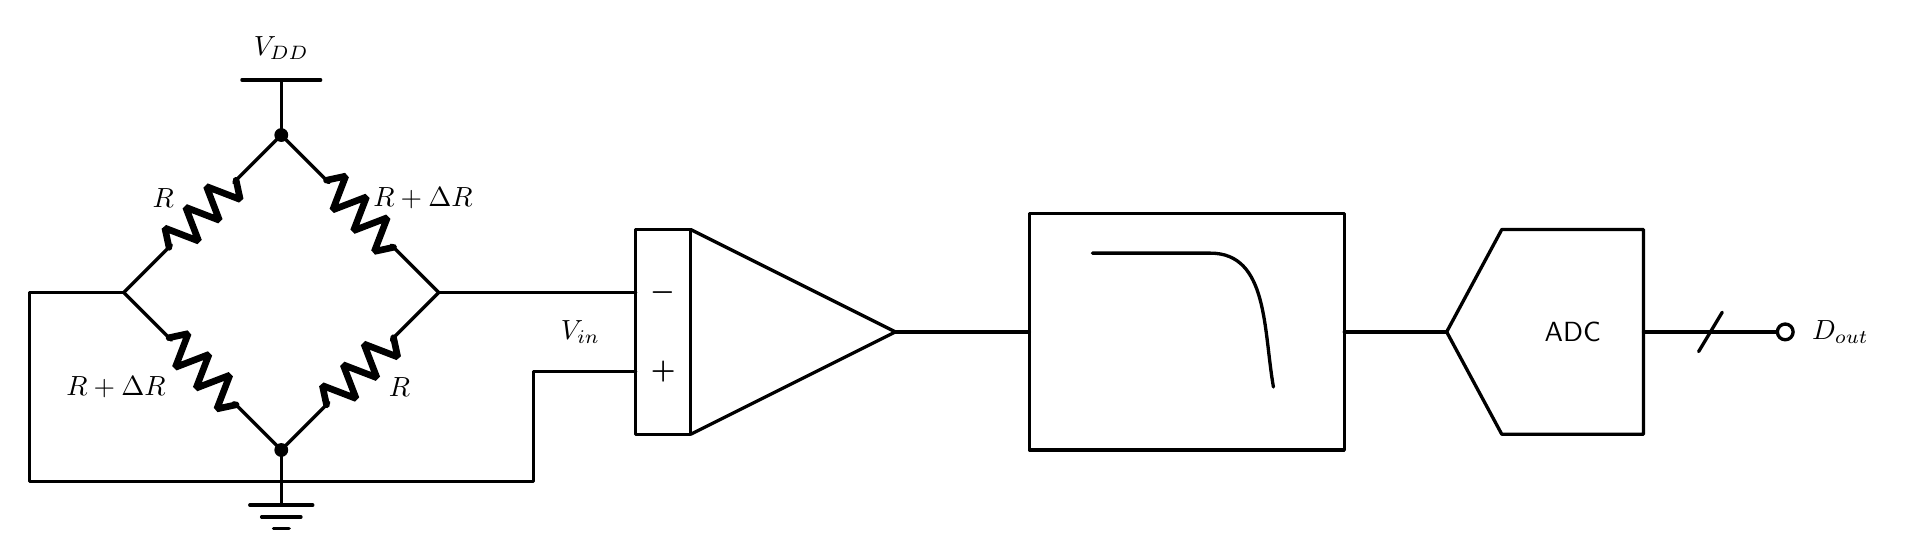
\begin{tikzpicture}[
    line width=1.2pt,
    line cap=round,
    line join=round
]
% 1. Wheatstone Bridge
\draw (-2,0) to[R] (0,2);
\draw (0,2) to[R] (2,0);
\draw (2,0) to[R] (0,-2);
\draw (0,-2) to[R] (-2,0);
\node at (-1.5, 1.2) {$R$};
\node at (1.8, 1.2) {$R + \Delta R$};
\node at (-2.1, -1.2) {$R + \Delta R$};
\node at (1.5, -1.2) {$R$};
\draw (0,2) -- (0,2.7);
\draw (-0.5, 2.7) -- (0.5, 2.7);
\node at (0, 3.1) {$V_{DD}$};
\fill (0,2) circle (2.5pt); 
\draw (0,-2) -- (0,-2.7);
\draw (-0.4, -2.7) -- (0.4, -2.7);
\draw (-0.25, -2.85) -- (0.25, -2.85);
\draw (-0.1, -3.0) -- (0.1, -3.0);
\fill (0,-2) circle (2.5pt); 

% 2. Instrumentation Amplifier
\draw (4.5, 0.8) rectangle (5.2, -1.8);
\draw (5.2, 0.8) -- (7.8, -0.5) -- (5.2, -1.8);
\node at (4.85, 0) {$\boldsymbol{-}$};
\node at (4.85, -1) {$\boldsymbol{+}$};

% 3. Lowpass filter
\draw (9.5, 1) rectangle (13.5, -2);
\draw (10.3, 0.5) -- (11.8, 0.5) to[out=0, in=100] (12.6, -1.2);

% 4. ADC
\draw (14.8, -0.5) -- (15.5, 0.8) -- (17.3, 0.8) -- (17.3, -1.8) -- (15.5, -1.8) -- cycle;
\node[font=\sffamily] at (16.4, -0.5) {ADC};

% 5. Routing
\draw (2,0) -- (4.5,0);
\draw (-2,0) -- (-3.2,0) -- (-3.2,-2.4) -- (3.2,-2.4) -- (3.2,-1) -- (4.5,-1);
\node at (3.8, -0.5) {$V_{in}$};
\draw (7.8, -0.5) -- (9.5, -0.5);
\draw (13.5, -0.5) -- (14.8, -0.5);
\draw (17.3, -0.5) -- (19, -0.5);
\draw[fill=white] (19.1, -0.5) circle (0.1);
\draw (18.0, -0.75) -- (18.3, -0.25);
\node at (19.8, -0.5) {$D_{out}$};
\end{tikzpicture}
}
\end{center}

\vspace{0.5em}
\begin{center}
\textbf{Figure 1. Strain gage signal condition architecture.}
\end{center}
\vspace{1em}

\textbf{Fig 1.} show the sensor signal conditioning ``front-end'' architecture for a strain gage sensor. The differential output voltage of the strain gage is amplified by the instrumentation amplifier and converted to a single-ended voltage. The output of the amplifier is fed to a lowpass filter which sets the noise bandwidth of the front-end circuitry.

The strain gage produces a differential output in response to an applied strain, which results from lengthening or shortening of a conductive element that changes its resistance. These changes in resistance are typically quite small, as the change in length $\Delta L$ relative to the nominal length $L$ is small, on the order of 0.1\% (for example).

Strain gage sensors are typically based on the Wheatstone bridge, a network of four resistances with an ``excitation voltage'' applied across the bridge ($V_{DD}$ in \textbf{Fig. 1}). The number of bridge resistances subjected to strain determines the strain gage sensitivity (expressed in mV/V).

\vspace{1.5em}
\textbf{\Large Phase 1}

For the first phase you are to design an instrumentation amplifier to amplify the strain gage signal while adding minimal noise. Filtering will be addressed during Phase 2 — for Phase 1 we will design assuming a signal bandwidth of $10 kHz$. \textbf{Fig. 2} shows the recommended architecture of the instrumentation amplifier.

\vspace{2em}
\begin{center}
\resizebox{0.85\textwidth}{!}{
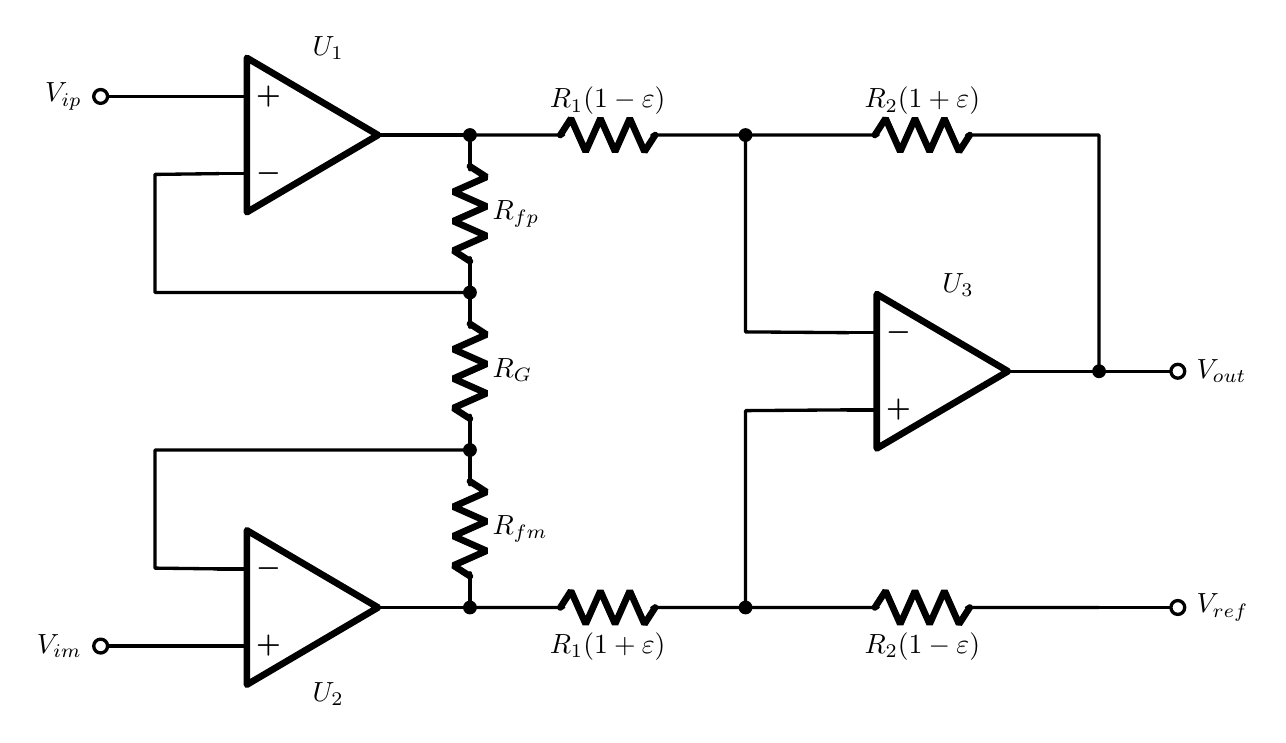
\begin{tikzpicture}[
    line width=1.2pt,
    line cap=round,
    line join=round
]
% Op-amps
\node[op amp, noinv input up] (U1) at (0, 3) {};
\node at (U1.center) [yshift=1.1cm, xshift=0.2cm] {$U_1$};
\node[op amp] (U2) at (0, -3) {};
\node at (U2.center) [yshift=-1.1cm, xshift=0.2cm] {$U_2$};
\node[op amp] (U3) at (8, 0) {};
\node at (U3.center) [yshift=1.1cm, xshift=0.2cm] {$U_3$};

% Input terminals
\draw (U1.+) -- ++(-1.5,0) coordinate (in_p);
\filldraw[fill=white, draw=black, line width=1.2pt] (in_p) circle (2.5pt);
\node[left] at (in_p) [xshift=-0.1cm] {$V_{ip}$};
\draw (U2.+) -- ++(-1.5,0) coordinate (in_m);
\filldraw[fill=white, draw=black, line width=1.2pt] (in_m) circle (2.5pt);
\node[left] at (in_m) [xshift=-0.1cm] {$V_{im}$};

% First stage
\draw (U1.out) -- (2, 3);
\draw (U2.out) -- (2, -3);
\draw (2, 3) to[R, l=$R_{fp}$] (2, 1);
\draw (2, 1) to[R, l=$R_G$] (2, -1);
\draw (2, -1) to[R, l=$R_{fm}$] (2, -3);
\fill (2, 3) circle (2.5pt);
\fill (2, 1) circle (2.5pt);
\fill (2, -1) circle (2.5pt);
\fill (2, -3) circle (2.5pt);
\draw (2, 1) -- (-2, 1) -- (-2, 2.5) -- (U1.-);
\draw (2, -1) -- (-2, -1) -- (-2, -2.5) -- (U2.-);

% Difference Amplifier Stage
\draw (2, 3) to[R, l=$R_1(1-\varepsilon)$] (5.5, 3);
\fill (5.5, 3) circle (2.5pt);
\draw (5.5, 3) -- (5.5, 0.5) -- (U3.-);
\draw (2, -3) to[R, l_=$R_1(1+\varepsilon)$] (5.5, -3);
\fill (5.5, -3) circle (2.5pt);
\draw (5.5, -3) -- (5.5, -0.5) -- (U3.+);

% Output & Reference
\draw (U3.out) -- ++(0.8,0) coordinate (out3);
\fill (out3) circle (2.5pt);
\draw (out3) -- ++(1.0,0) coordinate (v_out);
\filldraw[fill=white, draw=black, line width=1.2pt] (v_out) circle (2.5pt);
\node[right] at (v_out) [xshift=0.1cm] {$V_{out}$};
\draw (5.5, 3) to[R, l=$R_2(1+\varepsilon)$] (out3 |- 5.5, 3) -- (out3);
\draw (5.5, -3) to[R, l_=$R_2(1-\varepsilon)$] (out3 |- 5.5, -3) coordinate (v_ref_pre);
\draw (v_ref_pre) -- ++(1.0, 0) coordinate (v_ref);
\filldraw[fill=white, draw=black, line width=1.2pt] (v_ref) circle (2.5pt);
\node[right] at (v_ref) [xshift=0.1cm] {$V_{ref}$};
\end{tikzpicture}
}
\end{center}

\vspace{0.5em}
\begin{center}
\textbf{Figure 2. Instrumentation amplifier schematic.}
\end{center}
\vspace{2em}


\begin{center}
\renewcommand{\arraystretch}{1.8}
\begin{tabular}{p{3.5cm} c l}
\textbf{Parameter} & \textbf{Specification} & \textbf{Unit} \\
\hline
Supply \newline voltage \newline ($V_{DD}$) & $5$ & $V$ \\
Peak-to- \newline peak signal \newline amplitude & $20$ & $mV$ \\
Nominal \newline strain gage \newline resistance \newline ($R$) & $1$ & $k\Omega$ \\
Peak-to- \newline peak output \newline amplitude \newline ($V_{out}$) & $2$ & $V$ \\
Signal-to- \newline noise ratio & $\ge 77$ & $dB$ \\
Signal \newline bandwidth \newline ($f_{sbw}$) & $10$ & $kHz$ \\
Input- \newline referred \newline offset & $\le 1$ & $mV$ \\
CMRR & $90$ & $dB$ \\
Power \newline dissipation \newline ($I_{DD} \cdot V_{DD}$) & Optimize & $mW$ \\
Cost-per- \newline unit (10,000 \newline units) & Optimize & $\$$ \\
\end{tabular}
\end{center}

\vspace{2em}
\textbf{\Large Recommended design approach}

\begin{itemize}
    \setlength{\itemsep}{2pt}
    \item Determine the gain required to meet the output amplitude specification
    \item Determine the input-referred voltage noise density required to meet the SNR specification
    \item Perform noise analysis of the instrumentation amplifier and determine the relative impact of all noise sources on the input-referred noise. Be sure to include the noise from the strain gage resistance and opamp current noise. You should model the strain gage as its Thevenin equivalent circuit.
    \item Select component values that allow you to achieve the noise target, with resistor tolerances that make it possible to meet the CMRR specification
    \item It may be helpful to simulate with an ideal opamp first (e.g. UniversalOpamp2) to validate your calculations
    \item Use Digikey's or Analog Devices' component selection tables to select opamps that meet the requirements. Note that one limitation here is that the opamps you use have available SPICE models that include noise. Many of Analog Devices' models are already available in Ltspice. For any that aren't, you just need to import the SPICE netlist and create a new component (Ltspice will autogenerate the symbol for you, but you can also create a custom symbol).
    \item The common-mode rejection ratio (CMRR) will depend on the resistor matching in the second stage of the instrumentation amplifier. It is given by the expression
    
    $$ CMRR = CMRR_1 \times CMRR_2 = G_1 \times \frac{G_2 + 1}{4 \times \epsilon} $$
    
    \item where $G_1$ is the gain of the first stage, $G_2$ is the gain of the second stage, and $\epsilon$ is the tolerance of the resistors in the second stage
    \item $V_{ref}$ should be generated using a voltage buffer (don't use an ideal voltage source)
    \item Take a systematic approach, rather than trying to simulate the amplifier straight away and ``guess'' at the component values
\end{itemize}

\vspace{1.5em}
\textit{Note on supply voltage and input range:} You need to ensure that both the single-ended supply voltage of $5V$ and the nominal sensor output voltage ($5V/2 = 2.5V$) are compatible with your opamp selection(s).

\vspace{1em}
\textit{Flicker (1/f) noise:} Some CMOS opamps exhibit particularly high $1/f$ corner frequencies ($f_c$), which can significantly degrade your SNR. This can often be seen by the $e_{np-p}$ parameter provided in many datasheets (or the `0.1 to 10Hz VNoise' parameter in Analog Devices' opamp selection table). If your noise simulation result seems higher than expected, make sure your noise isn't being dominated by flicker noise.

\vspace{2em}
\textbf{\Large Phase 1 deliverables}

Jupyter Notebook detailing the following:

\begin{enumerate}
    \setlength{\itemsep}{2pt}
    \item Input-referred noise target derived from the specifications. Include a discussion on how you arrived at this value.
    \item Expression showing the relative contribution of each noise source on the input-referred noise. Justify any assumptions.
    \item Complete schematic showing the strain gage model, supply voltages, opamp models, resistor values, and DC operating point voltages at all nodes
    \item Table showing components used, quantitiy, and cost per unit (assuming a total of 10,000 units)
    \item AC simulation results showing the differential frequency response of the amplifier
    \item AC simulation results showing the \textit{common-mode} frequency response of the amplifier with resistor mismatch. The worst-case mismatch condition is depicted in \textbf{Fig. 2}.
    \item Input-referred noise plot showing the input-referred noise density at 10kHz, as well as integrated noise from 0.1Hz to 10kHz (this should show that your design will meet spec once you add a filter).
\end{enumerate}

\vspace{2em}
\noindent
\texttt{\color{blue!80!black}In [~]:} \framebox[0.9\textwidth]{\rule{0pt}{15pt}}

\end{document}